\documentclass[border=6pt]{standalone}
%=======================================================================
%  ICCIT 2026 -- CAMERA-READY version, 6 pages, IEEE conference format
%  From Spikes to Sentences: A Hybrid CTC Decoder with Confidence-Gated
%  Language Model Rescoring
%  Compile: pdflatex x3, with revision_results.tex in this folder.
%=======================================================================

\usepackage{amsmath,amssymb}
\usepackage{graphicx}
\usepackage{booktabs}
\usepackage{multirow}
\usepackage{array}
\usepackage{xcolor}
\usepackage{tikz}
\usetikzlibrary{arrows.meta,positioning,calc,fit,backgrounds,shapes.geometric}
\usepackage{pgfplots}
\pgfplotsset{compat=1.17}
\usepackage{algorithm}
\usepackage{algpseudocode}
\usepackage{adjustbox}



\definecolor{ioFill}{HTML}{ECEFF4}\definecolor{ioLine}{HTML}{4C566A}
\definecolor{acFill}{HTML}{E3EEF9}\definecolor{acLine}{HTML}{3B6EA5}
\definecolor{reFill}{HTML}{E0F0EC}\definecolor{reLine}{HTML}{2E8B7F}
\definecolor{trFill}{HTML}{ECE6F5}\definecolor{trLine}{HTML}{6A4C93}
\definecolor{deFill}{HTML}{E6F0E1}\definecolor{deLine}{HTML}{4E8B3B}
\definecolor{llFill}{HTML}{FBEBDD}\definecolor{llLine}{HTML}{C1662F}
\definecolor{gaFill}{HTML}{FFF6E9}\definecolor{gaLine}{HTML}{B8860B}
\definecolor{inkLine}{HTML}{3B4252}

\tikzset{
  blk/.style={rounded corners=3pt,draw,line width=0.9pt,align=center,
              inner sep=4pt,font=\footnotesize},
  io/.style={blk,fill=ioFill,draw=ioLine},
  ac/.style={blk,fill=acFill,draw=acLine},
  re/.style={blk,fill=reFill,draw=reLine},
  tr/.style={blk,fill=trFill,draw=trLine},
  de/.style={blk,fill=deFill,draw=deLine},
  ll/.style={blk,fill=llFill,draw=llLine},
  gate/.style={diamond,aspect=1.7,draw=gaLine,fill=gaFill,line width=0.9pt,
               align=center,inner sep=1pt,font=\footnotesize},
  fl/.style={-{Stealth[length=5pt]},line width=0.9pt,draw=inkLine},
  dec/.style={-{Stealth[length=5pt]},line width=0.8pt,draw=deLine,dashed},
  tag/.style={font=\scriptsize\itshape,text=inkLine,fill=white,inner sep=1pt},
  capt/.style={font=\scriptsize,text=ioLine},
}

\newcommand{\pct}{\,\%}


\begin{document}
\setlength{\columnwidth}{3.5in}
\fontsize{10}{12}\selectfont
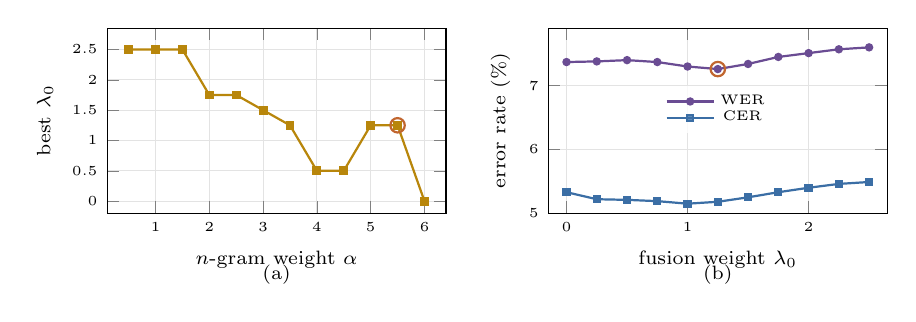
\begin{tikzpicture}
\begin{axis}[
  name=pA,
  width=0.355\columnwidth, height=2.35cm, scale only axis,
  xlabel={$n$-gram weight $\alpha$}, ylabel={best $\lambda_0$},
  xmin=0.1, xmax=6.4, ymin=-0.2, ymax=2.85,
  xtick={1,2,3,4,5,6}, ytick={0,0.5,1.0,1.5,2.0,2.5},
  yticklabel style={/pgf/number format/fixed,
                    /pgf/number format/precision=2},
  tick label style={font=\tiny}, label style={font=\scriptsize},
  grid=major, grid style={gray!22},
]
\addplot[color=gaLine,mark=square*,mark size=1.2pt,line width=0.8pt]
  coordinates {(0.5,2.50)(1.0,2.50)(1.5,2.50)(2.0,1.75)(2.5,1.75)(3.0,1.50)
               (3.5,1.25)(4.0,0.50)(4.5,0.50)(5.0,1.25)(5.5,1.25)(6.0,0.00)};
\addplot[only marks,mark=o,mark size=2.6pt,color=llLine,line width=0.8pt]
  coordinates {(5.5,1.25)};
\end{axis}

\begin{axis}[
  name=pB,
  width=0.355\columnwidth, height=2.35cm, scale only axis,
  at={($(pA.east)+(1.30cm,0)$)}, anchor=west,
  xlabel={fusion weight $\lambda_0$}, ylabel={error rate (\%)},
  xmin=-0.15, xmax=2.65, ymin=5.0, ymax=7.9,
  xtick={0,1,2}, ytick={5,6,7},
  tick label style={font=\tiny}, label style={font=\scriptsize},
  legend style={font=\tiny,at={(0.50,0.56)},anchor=center,draw=none,
                fill=white,fill opacity=0.8,text opacity=1,row sep=-3pt,
                inner sep=1pt},
  grid=major, grid style={gray!22},
]
\addplot[color=trLine,mark=*,mark size=1.1pt,line width=0.8pt]
  coordinates {(0,7.37)(0.25,7.38)(0.5,7.40)(0.75,7.37)(1.0,7.30)(1.25,7.26)
               (1.5,7.34)(1.75,7.45)(2.0,7.51)(2.25,7.57)(2.5,7.60)};
\addlegendentry{WER}
\addplot[color=acLine,mark=square*,mark size=1.1pt,line width=0.8pt]
  coordinates {(0,5.33)(0.25,5.22)(0.5,5.21)(0.75,5.19)(1.0,5.15)(1.25,5.18)
               (1.5,5.25)(1.75,5.33)(2.0,5.40)(2.25,5.46)(2.5,5.49)};
\addlegendentry{CER}
\addplot[only marks,mark=o,mark size=2.6pt,color=llLine,line width=0.8pt]
  coordinates {(1.25,7.26)};
\end{axis}
\node[font=\scriptsize] at ($(pA.south)+(0,-0.78cm)$) {(a)};
\node[font=\scriptsize] at ($(pB.south)+(0,-0.78cm)$) {(b)};
\end{tikzpicture}
\end{document}
